\documentclass[a4paper]{article}
\usepackage{cmap}
\usepackage{mathtext}
\usepackage{amssymb}
\usepackage{amsmath}
\usepackage[russian]{babel}
\usepackage{indentfirst}
\usepackage[pdftex]{graphicx}
\usepackage{multirow}
\usepackage{mathrsfs}
\usepackage{biblatex}
\usepackage{siunitx}
\usepackage[left=2cm,right=2cm,top=2cm,bottom=2cm]{geometry}
\usepackage{fancyhdr}
\bibliography{bib}
\pagestyle{fancy}
\newcommand{\const}{\mathrm{const}}
\newcommand{\rref}[1]{(\ref{#1})}
\newenvironment{comment}{}{}
\newcommand{\picref}[1]{рис. \ref{#1}}
\newcommand{\mbf}{\mathbf}
\newcommand{\Equip}[3]{
	
	{\bf #1:} $\Delta = \pm #2\; #3$}
\newcommand{\equip}[1]{
	
	{\bf #1}}
\newcommand{\labname}{Исследование разрешающей способности микроскопа методом Аббе} 	% название пиши здесь
\newcommand{\labnum}{4.3.3}		% номер вводи здесь без точки
\fancyfoot{}
\fancyhead[RE, RO]{\thepage}
\fancyhead[LE, LO]{Лабораторная работа \labnum \space \labname}
\title{Лабораторная работа \labnum \space \labname}
\author{Иван Сладков}
\begin{document}
\maketitle
\thispagestyle{empty}
\section{Аннотация}

В данной работе проводится определение периода решёток по их пространственному спектру и по увеличенному изображению, а также определение дифракционного предела разрешения объектива микроскопа методом Аббе. Кроме того, исследуются пространственная фильтрация и мультипликация изображения решётки.

\section{Теоретические сведения}

\paragraph{Принцип двойной дифракции и формирование оптического	изображения.}

Формирование изображения с помощью линзы можно рассматривать, основываясь на идее пространственного спектрального разложения. Монохроматическую волну, идущую от предмета, представим в виде суперпозиции плоских волн разных направлений $ \alpha $, т. е. разных пространственных частот $ u = k \sin \alpha $. Каждая гармоника фокусируется линзой в определённую точку фокальной плоскости, и там возникает картина пространственного спектра. По этой причине фокальную плоскость линзы называют фурье-плоскостью.

В процессе распространения света от предмета до фурье-плоскости осуществляется преобразование Фурье светового поля (по терминологии Аббе -- первая дифракция). Процесс распространения света от фурье-плоскости до плоскости изображения (рис. \ref{fig:screenshot1}) -- вторая дифракция.

Можно сказать, что в процессе образования изображения происходит два последовательных преобразования Фурье: от входной плоскости $ П_1 $ к фурье-плоскости -- первая дифракция, и затем от фурье-плоскости с помощью линзы $ Л_2 $ к выходной плоскости $ П_2 $ -- вторая дифракция.


\begin{figure}[tbp]
	\centering
	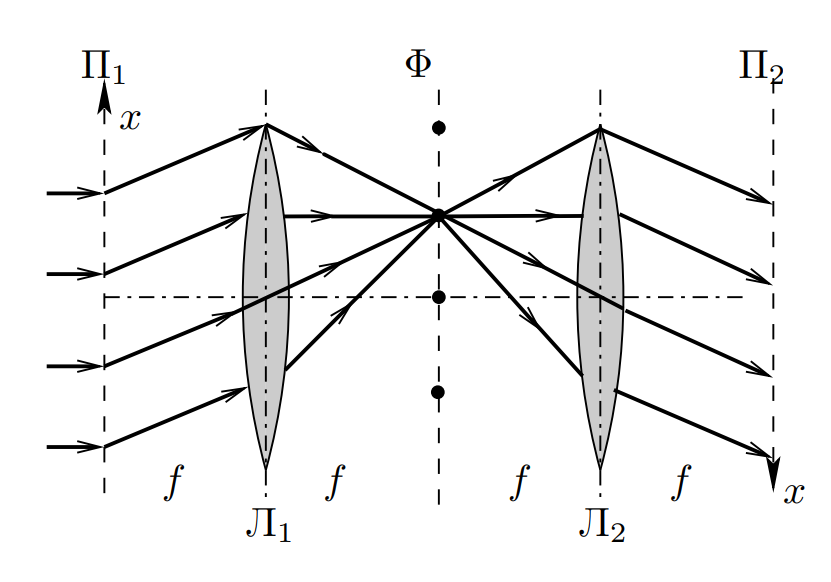
\includegraphics[width=0.8\linewidth]{Screenshot_1}
	\caption{Двойная дифракция Аббе}
	\label{fig:screenshot1}
\end{figure}

\paragraph{Пространственная фильтрация.}

В фурье-плоскости возможно избирательное воздействие на разные пространственные гармоники: установив в любой точке $ x $ этой плоскости пластинку, вносящую определённое поглощение, мы изменим амплитуду и фазу плоской волны с пространственной частотой $ u = k x / f $, не изменяя амплитуд и фаз других плоских волн.

\paragraph{Мультипликация изображения.}

Изображение, возникающее в плоскости $ П_2 $, представляет собой периодически повторяющееся с периодом $$ d_0 = \lambda f / d $$ изображение объекта с функцией пропускания $ f_0 (x) $.
Соседние элементы периодической структуры, видимой в $ П_2, $ $ f(x) = \Sigma f_0(x-n d_0) $, не налагаются друг на друга при условии $ d_0 > a $, где $ a $ -- размер объекта. Число элементов $ N $ размноженного изображения определяется шириной главного максимума картины дифракции Фраунгофера на отдельной щели решётки: $$ N\approx 2 b / d_0. $$

\paragraph{Разрешающая способность. Критерий Рэлея.} 

Согласно качественному критерию, предложенному Рэлеем, два источника света различимы, если дифракционный максимум одного приходится на минимум другого. Т. е, расстояние между центрами пятен $ \Delta x $ равно полуширине пятна Эйри (рис. \ref{fig:screenshot2}): \[\Delta x = 1.22 \frac{\lambda}{D} z,\] где $ z $ -- расстояние от диафрагмы до плоскости наблюдения, а $ D $ -- диаметр диафрагмы. Отсюда минимальное угловое разрешение равно: \[\alpha_{min} \approx 1.22 \frac{\lambda}{D}.\]

\begin{figure}[tbp]
	\centering
	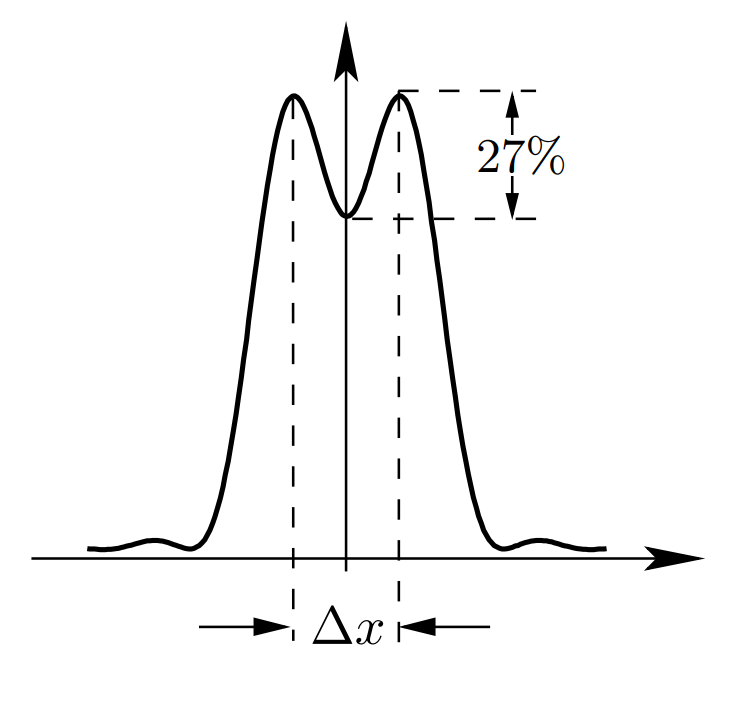
\includegraphics[width=0.8\linewidth]{Screenshot_2}
	\caption{Разрешение двух пятен Эйри}
	\label{fig:screenshot2}
\end{figure}


\subsection{Расчётные формулы}

Минимально разрешаемое объективом расстояние:
\begin{equation}\label{минимальное_расстояние}
	l_{min}\approx \frac{2 f \lambda}{D},
\end{equation}
где $ f $ -- фокусное расстояние линзы.

Условия главных максимумов:
\begin{equation}\label{условие_максимумов}
	d \sin \theta_x = m_x \lambda, \;\;\;	d \sin \theta_y = m_y \lambda,
\end{equation}
где $ m_{x, y} $ -- порядок дифракционных максимумов.

Увеличение системы собирающих линз (в условиях опыта):
\begin{equation}\label{увеличение}
	\Gamma = \frac{b_1 b_2}{a_1 a_2},
\end{equation}
где $ a, \; b $ -- соответствующие расстояния на рис. \ref{fig:screenshot3}.

\section{Оборудование и инструментальные погрешности}

Схема экспериментальной установки отображена на рис. \ref{fig:screenshot3}. Излучение лазера (ОКГ) почти перпендикулярно падает на сетку С, установленную вблизи фокальной плоскости линзы $ Л_1 $ — объектива. Вторичное изображение из плоскости $ P_2 $ проецируется на экран Э линзой $ Л_2 $.


\begin{figure}[tbp]
	\centering
	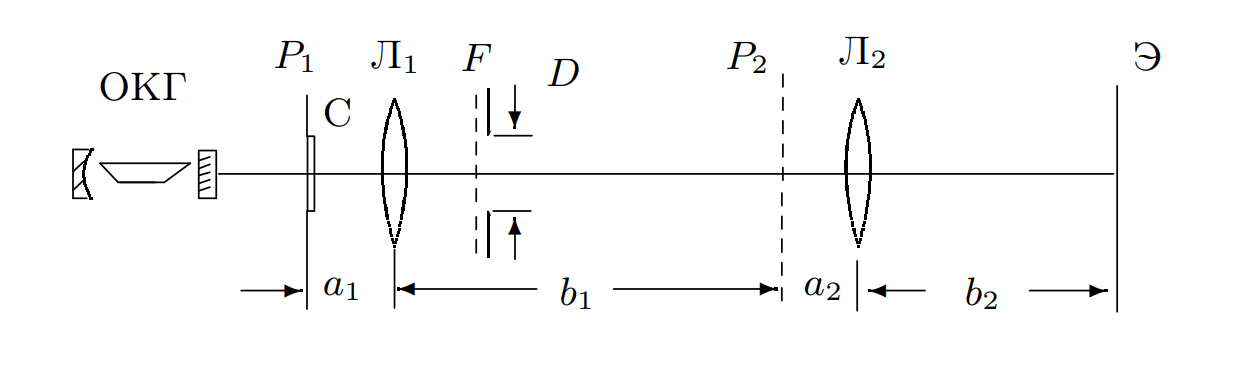
\includegraphics[width=0.8\linewidth]{Screenshot_3}
	\caption{Схема экспериментальной установки}
	\label{fig:screenshot3}
\end{figure}

В работе используются:
\equip{Лазер}: $ \lambda = 532 \; нм $
\equip{Кассета с набором сеток}
\equip{Линзы}: $ f_1 = 110 \; мм; \; f_2 = 25\; мм $
\equip{Щель с микрометрическим винтом}
\equip{Оптический стол}
\equip{Экран}
\Equip{Линейка}{0.5}{мм}
\equip{Светофильтр}

\section{Результаты измерений и обработка данных}
\emph{Все измерения и расчёты в СИ.}

\subsection{Определение периода решёток}

Расстояние от сетки до экрана: $ H = 142\pm 0.5 \; см. $ 
Из формул (\ref{условие_максимумов}), где $ \sin \theta \sim a / H $ и $ a $ -- период изображения, получим результат в табл. \ref{tab:спектр}.

\begin{table}[h]
	\centering
	\begin{tabular}{|l|l|l|l|l|l|l|}
		\hline
		$n$ & $a$  & $\delta_a$ & $H$  & $\delta_H$ & $d$     & $\delta_d$ \\ \hline
		2   & 38   & 0.5        & 1420 & 5          & 0.0198 & 0.0001    \\ \hline
		3   & 25   & 0.5        & 1420 & 5          & 0.0302 & 0.0003    \\ \hline
		4   & 12.5 & 0.5        & 1420 & 5          & 0.060 & 0.001    \\ \hline
		5   & 6.25 & 0.5        & 1420 & 5          & 0.120 & 0.005      \\ \hline
		6   & 4.6  & 0.5        & 1420 & 5          & 0.16 & 0.01    \\ \hline
	\end{tabular}
	\caption{Определение периода по картине спектра}
	\label{tab:спектр}
\end{table}
\newpage
Теперь соберём микроскоп с параметрами:
\[a_1 = 13.5\pm 0.5\; см,\]
\[b_1 = 48\pm 0.5\; см,\]
\[a_2 = 2.5\pm 0.1\; см,\]
\[b_2 = 59\pm 0.5\; см.\]

По формуле (\ref{увеличение}), $ \Gamma = 84\pm 5 $. Тогда найдём период решётки (табл. \ref{tab:изображение}).

\begin{table}[h]
	\centering
	\begin{tabular}{|l|l|l|l|l|l|l|}
		\hline
		$n$ & $a$ & $\delta_a$ & $\Gamma$ & $\delta_\Gamma$ & $d$  & $\delta_d$ \\ \hline
		2   & --- & ---        & ---      & ---             & ---  & ---        \\ \hline
		3   & 3.9 & 0.5        & 85       & 5               & 0.04 & 0.01       \\ \hline
		4   & 5.9 & 0.5        & 85       & 5               & 0.07 & 0.01       \\ \hline
		5   & 12  & 0.5        & 85       & 5               & 0.14 & 0.015      \\ \hline
		6   & 16  & 0.5        & 85       & 5               & 0.18 & 0.02       \\ \hline
	\end{tabular}
	\caption{Определение периода по увеличенному изображению}
	\label{tab:изображение}
\end{table}

Далее по формуле (\ref{минимальное_расстояние}) найдём период решётки через критерий Рэлея. Результаты в табл. \ref{tab:разрешение}.

\begin{table}[h]
	\centering
	\begin{tabular}{|l|l|l|l|l|l|}
		\hline
		$n$ & $D$   & $\delta_D$ & $f$ & $d$    & $\delta_d$ \\ \hline
		2   & ---   & ---        & --- & ---    & ---        \\ \hline
		3   & 3.35  & 0.01       & 110 & 0.0349 & 1E-4       \\ \hline
		4   & 1.95  & 0.01       & 110 & 0.0600 & 3E-4       \\ \hline
		5   & 1     & 0.01       & 110 & 0.117  & 0.001      \\ \hline
		6   & 0.695 & 0.01       & 110 & 0.168  & 0.003      \\ \hline
	\end{tabular}
	\caption{Определение периода по наименьшему разрешению}
	\label{tab:разрешение}
\end{table} 

\subsection{Пространственная фильтрация и мультипликация}

Убедились, что при пропускании через щель только максимумов $ (0, m_y) $ наблюдаются горизонтальные дифракционные полосы, а при $ (m_x, 0) $ -- вертикальные.

Если выставить щель под $ 45^\circ $ и пропускать $ (m_i, m_i) $ максимумы, наблюдаем наклонные полосы (рис. \ref{fig:img3264}).

\begin{figure}[tbp]
	\centering
	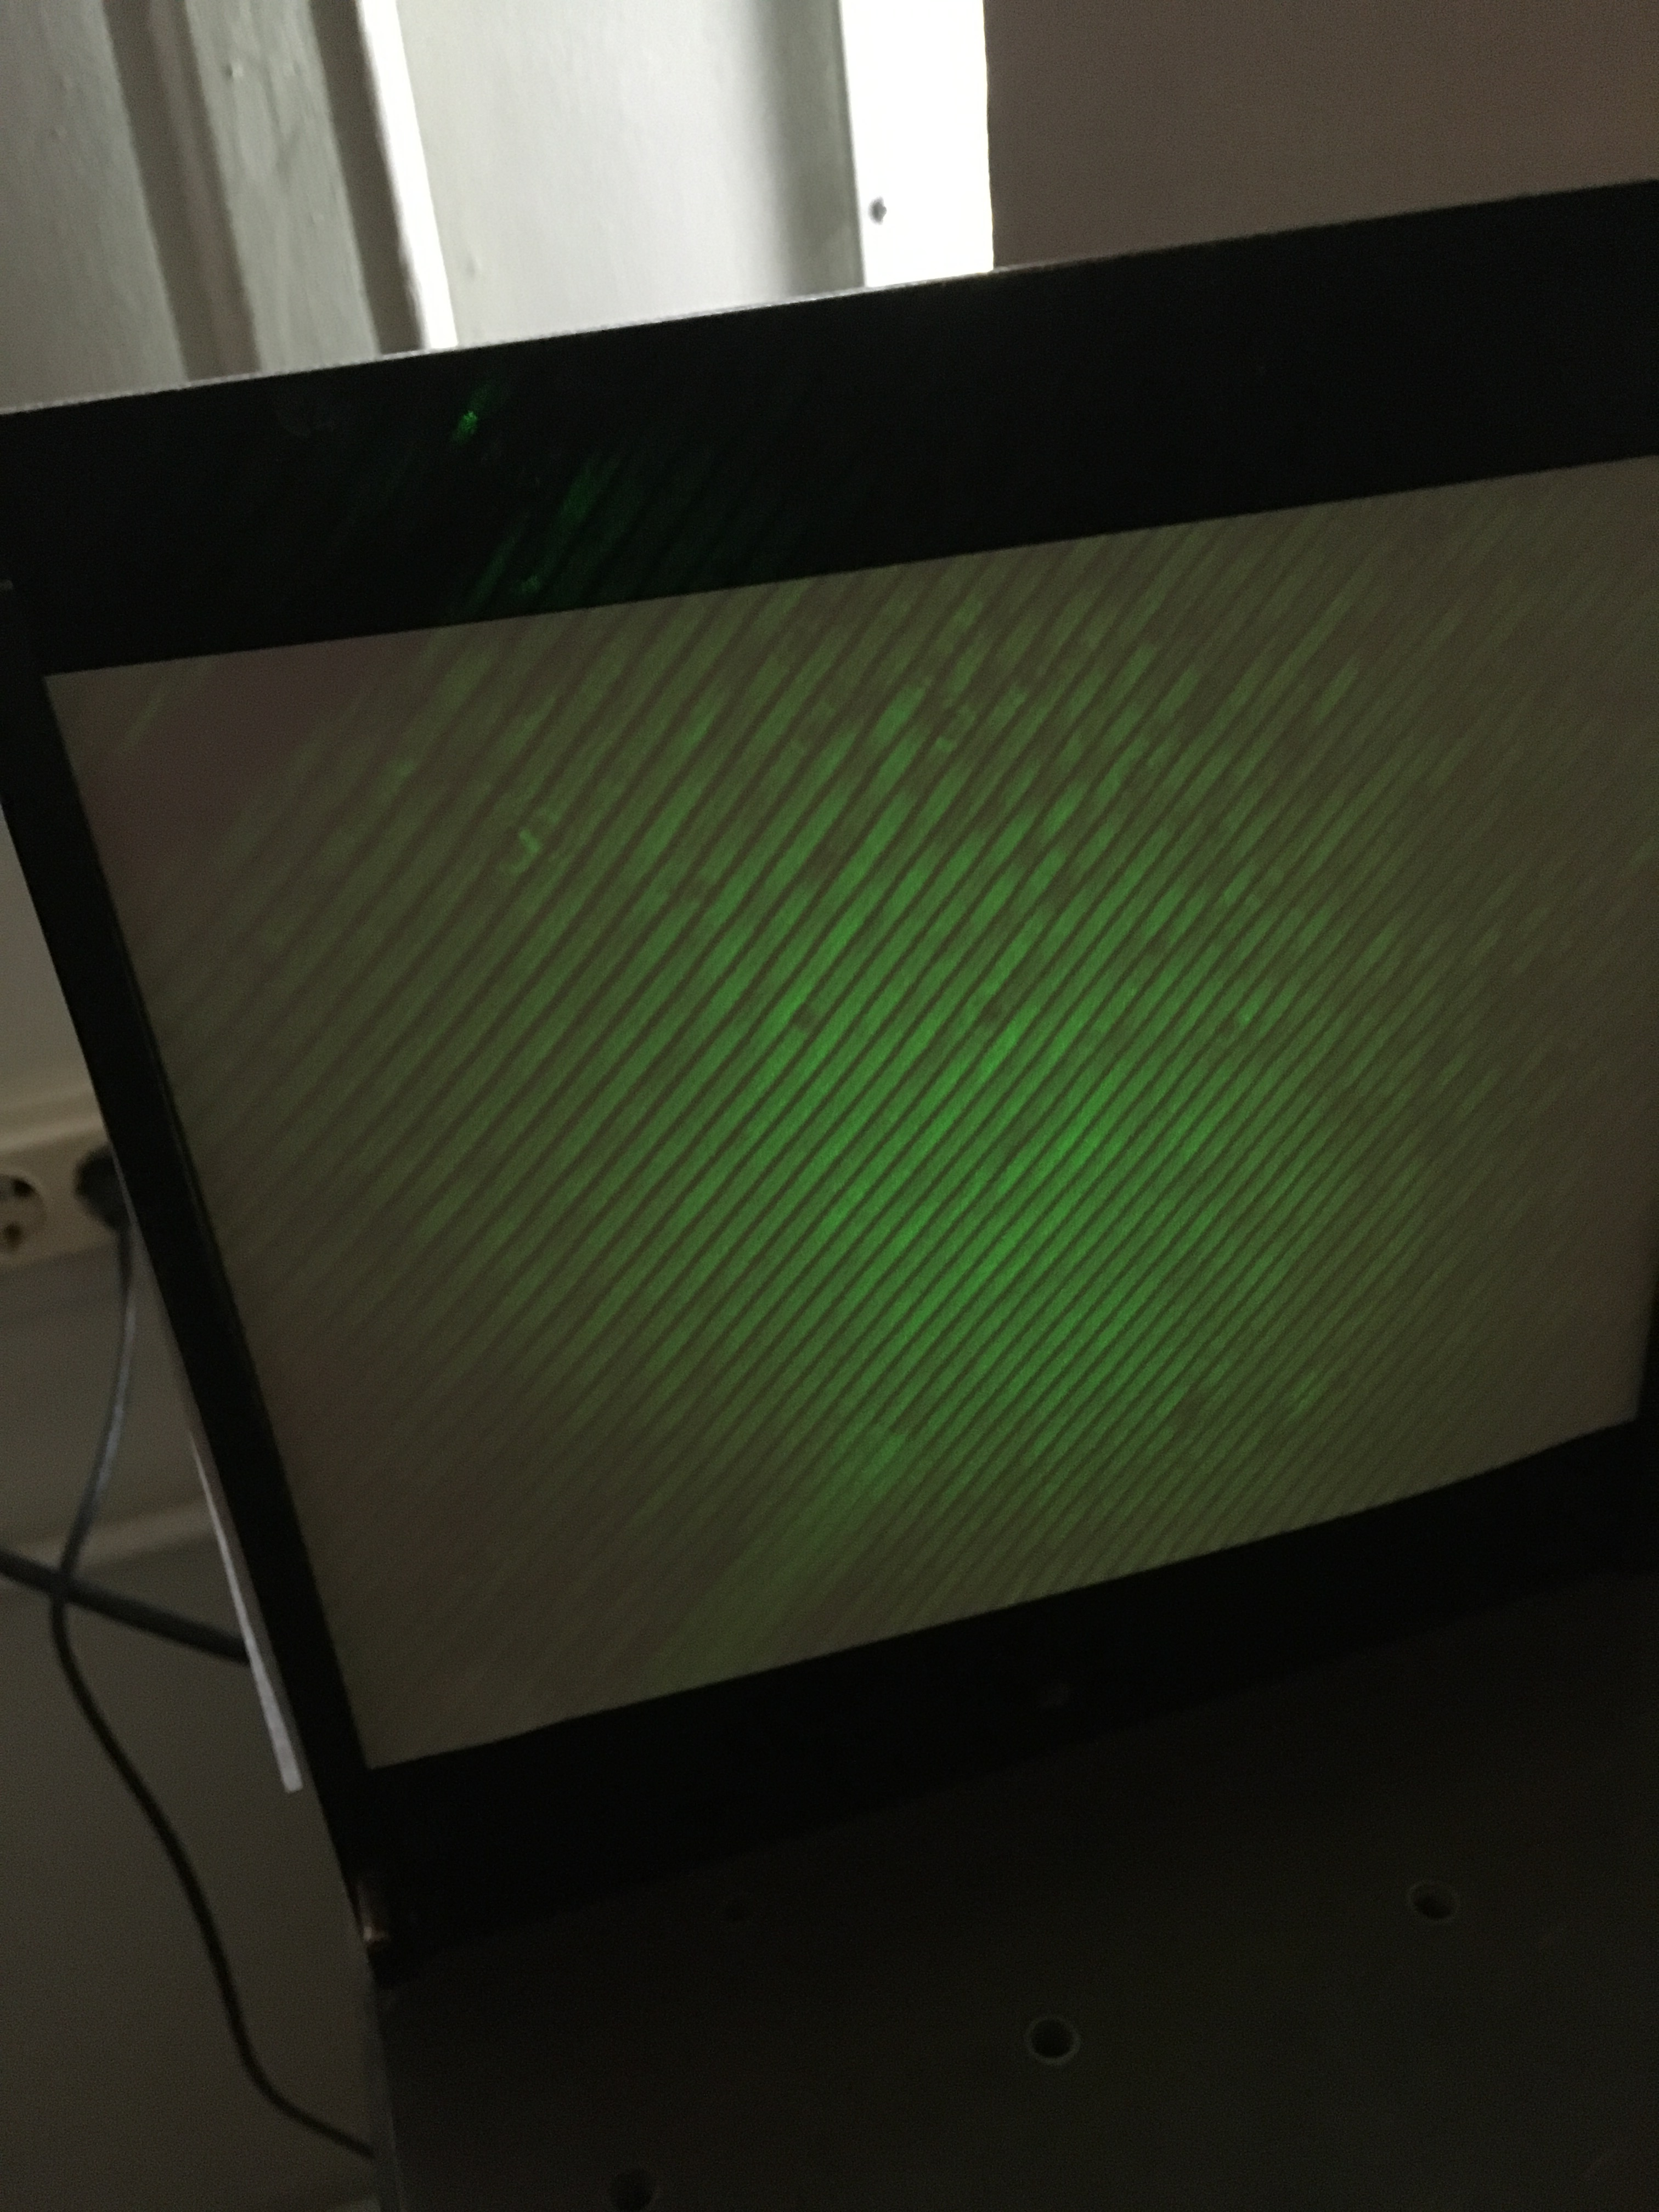
\includegraphics[height=0.4\textheight]{IMG_3264}
	\caption{Дифракционная картина от максимумов $(m_i, m_i)$}
	\label{fig:img3264}
\end{figure}

Теперь исследуем мультиплицирование: при уменьшении периода сетки увеличивается период мультиплицированной картины на экране (рис. \ref{fig:мультипликация}); при увеличении щели увеличивается ширина каждого изображения. 

\begin{figure}[tbp]
	\centering
	\begin{minipage}{0.49\linewidth}
		\centering
		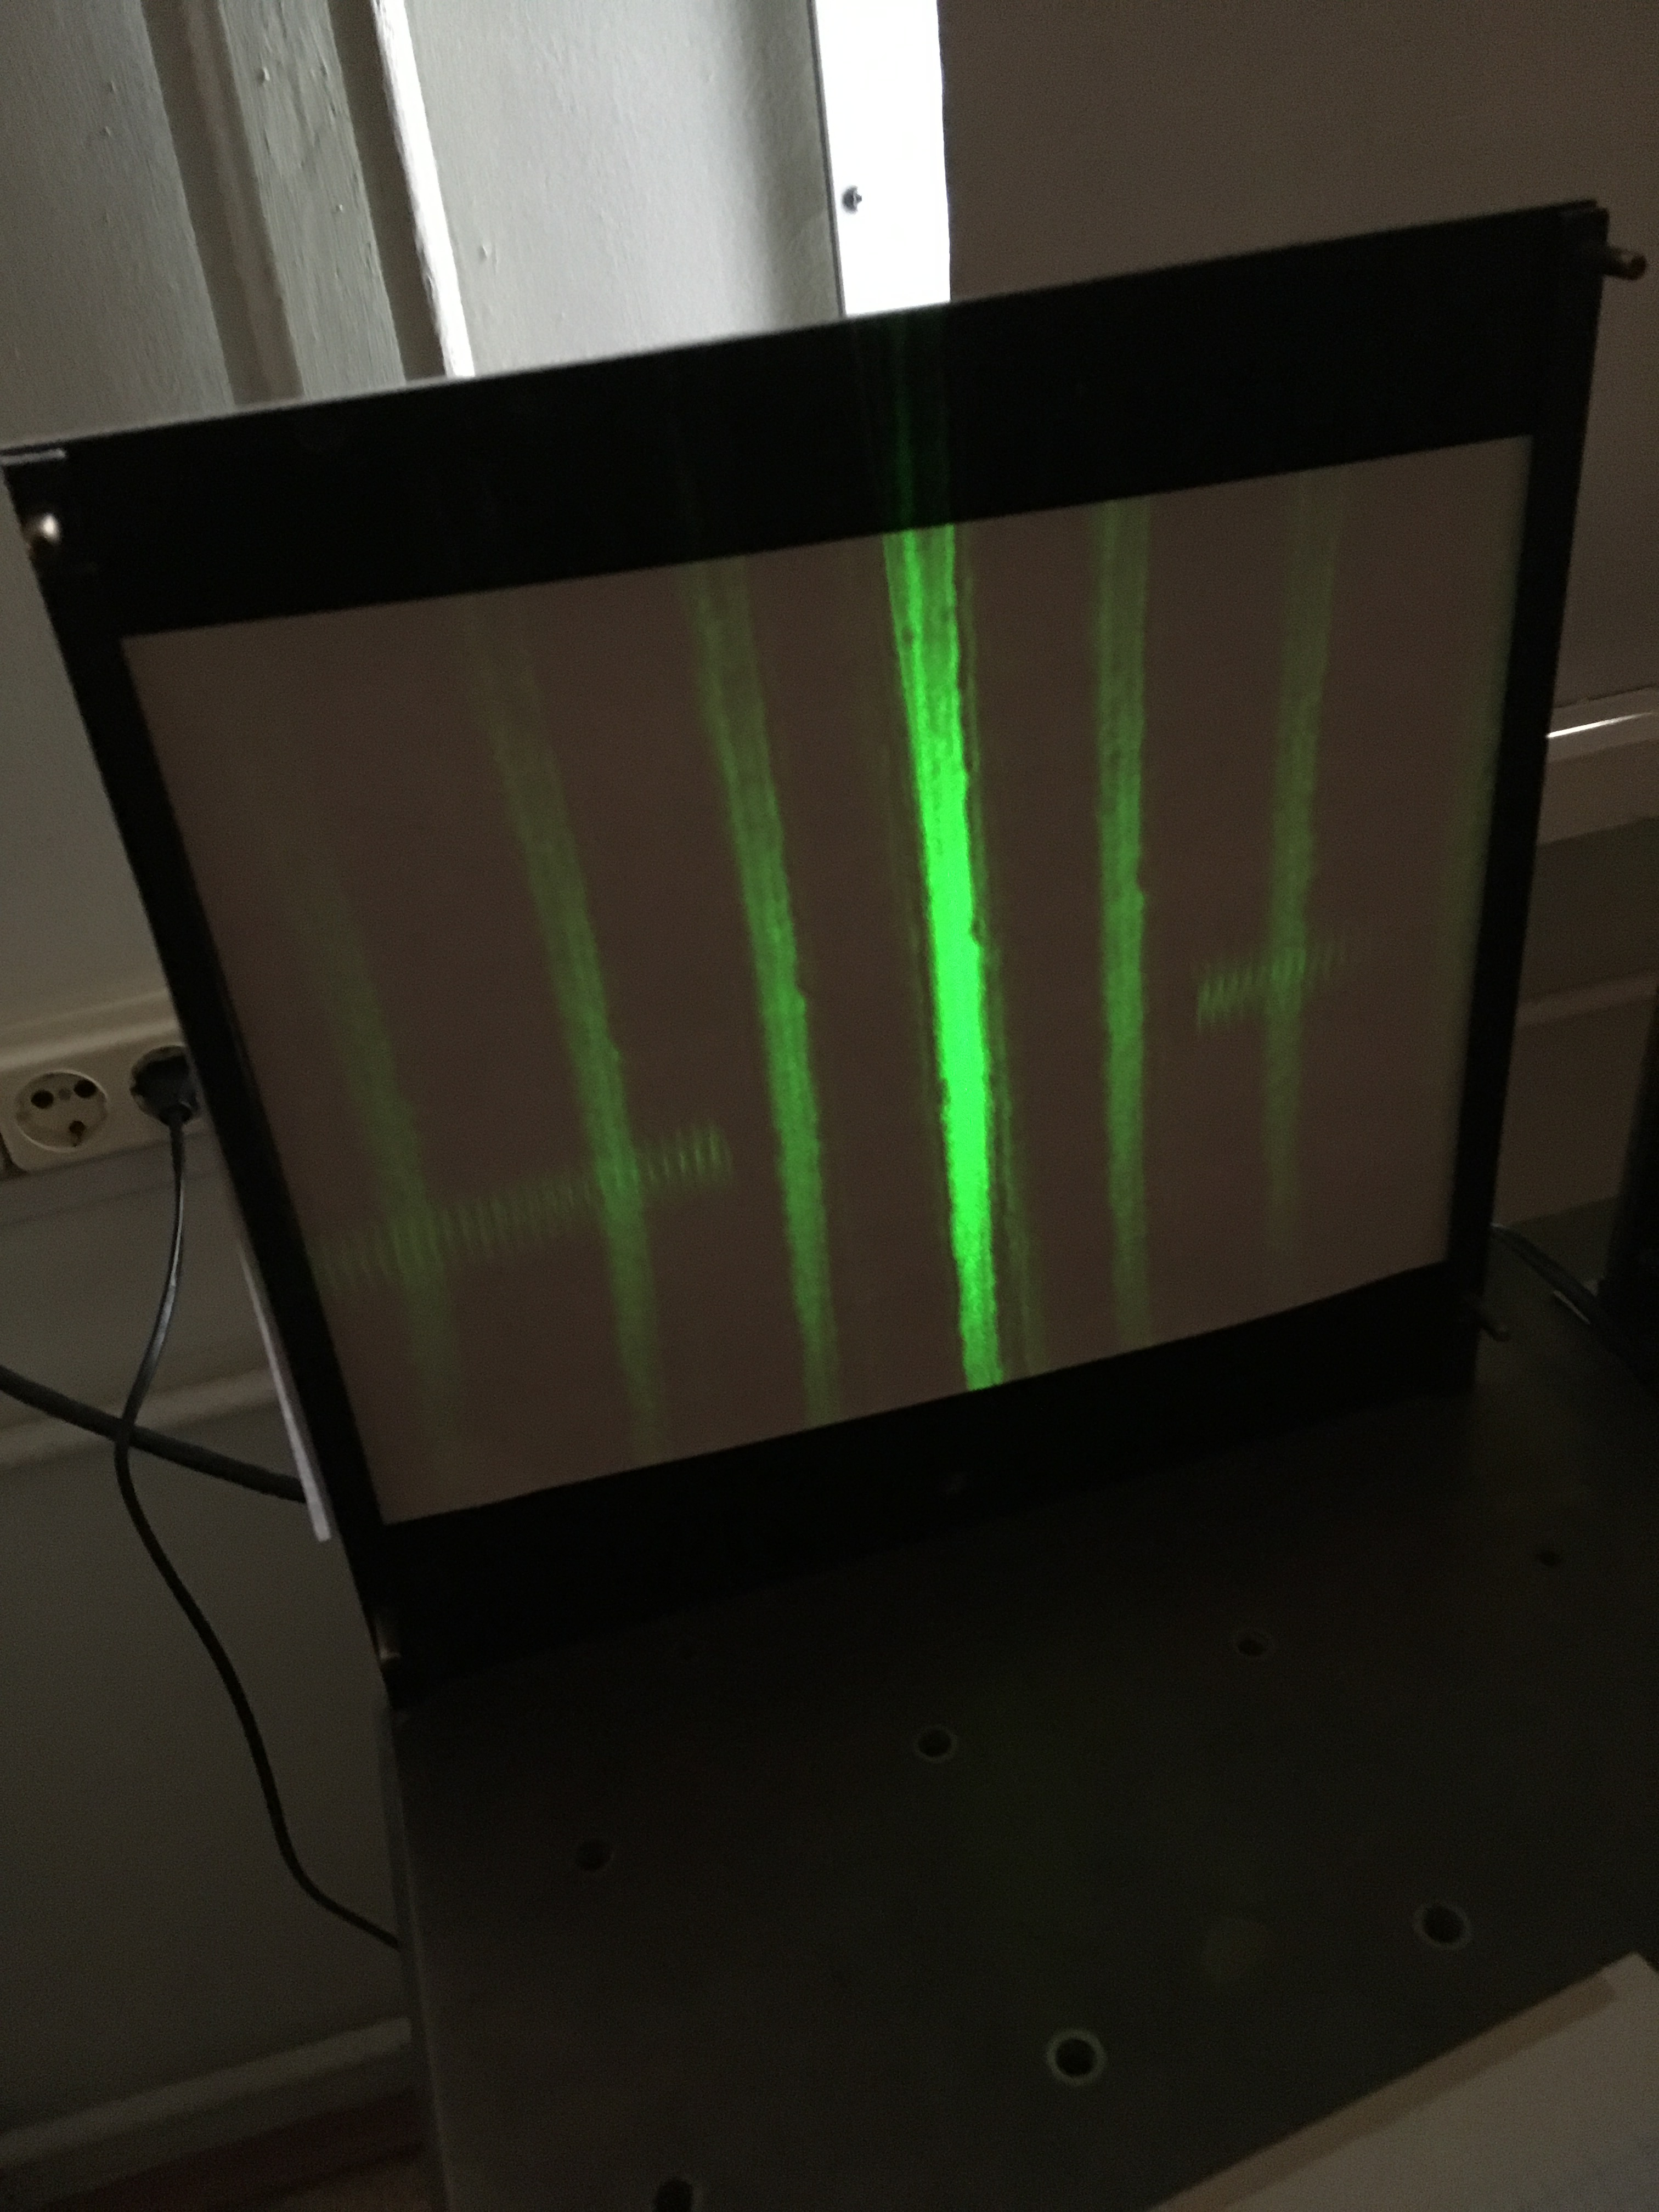
\includegraphics[width=0.8\linewidth]{IMG_3269}
	\end{minipage}
	\begin{minipage}{0.49\linewidth}
		\centering
		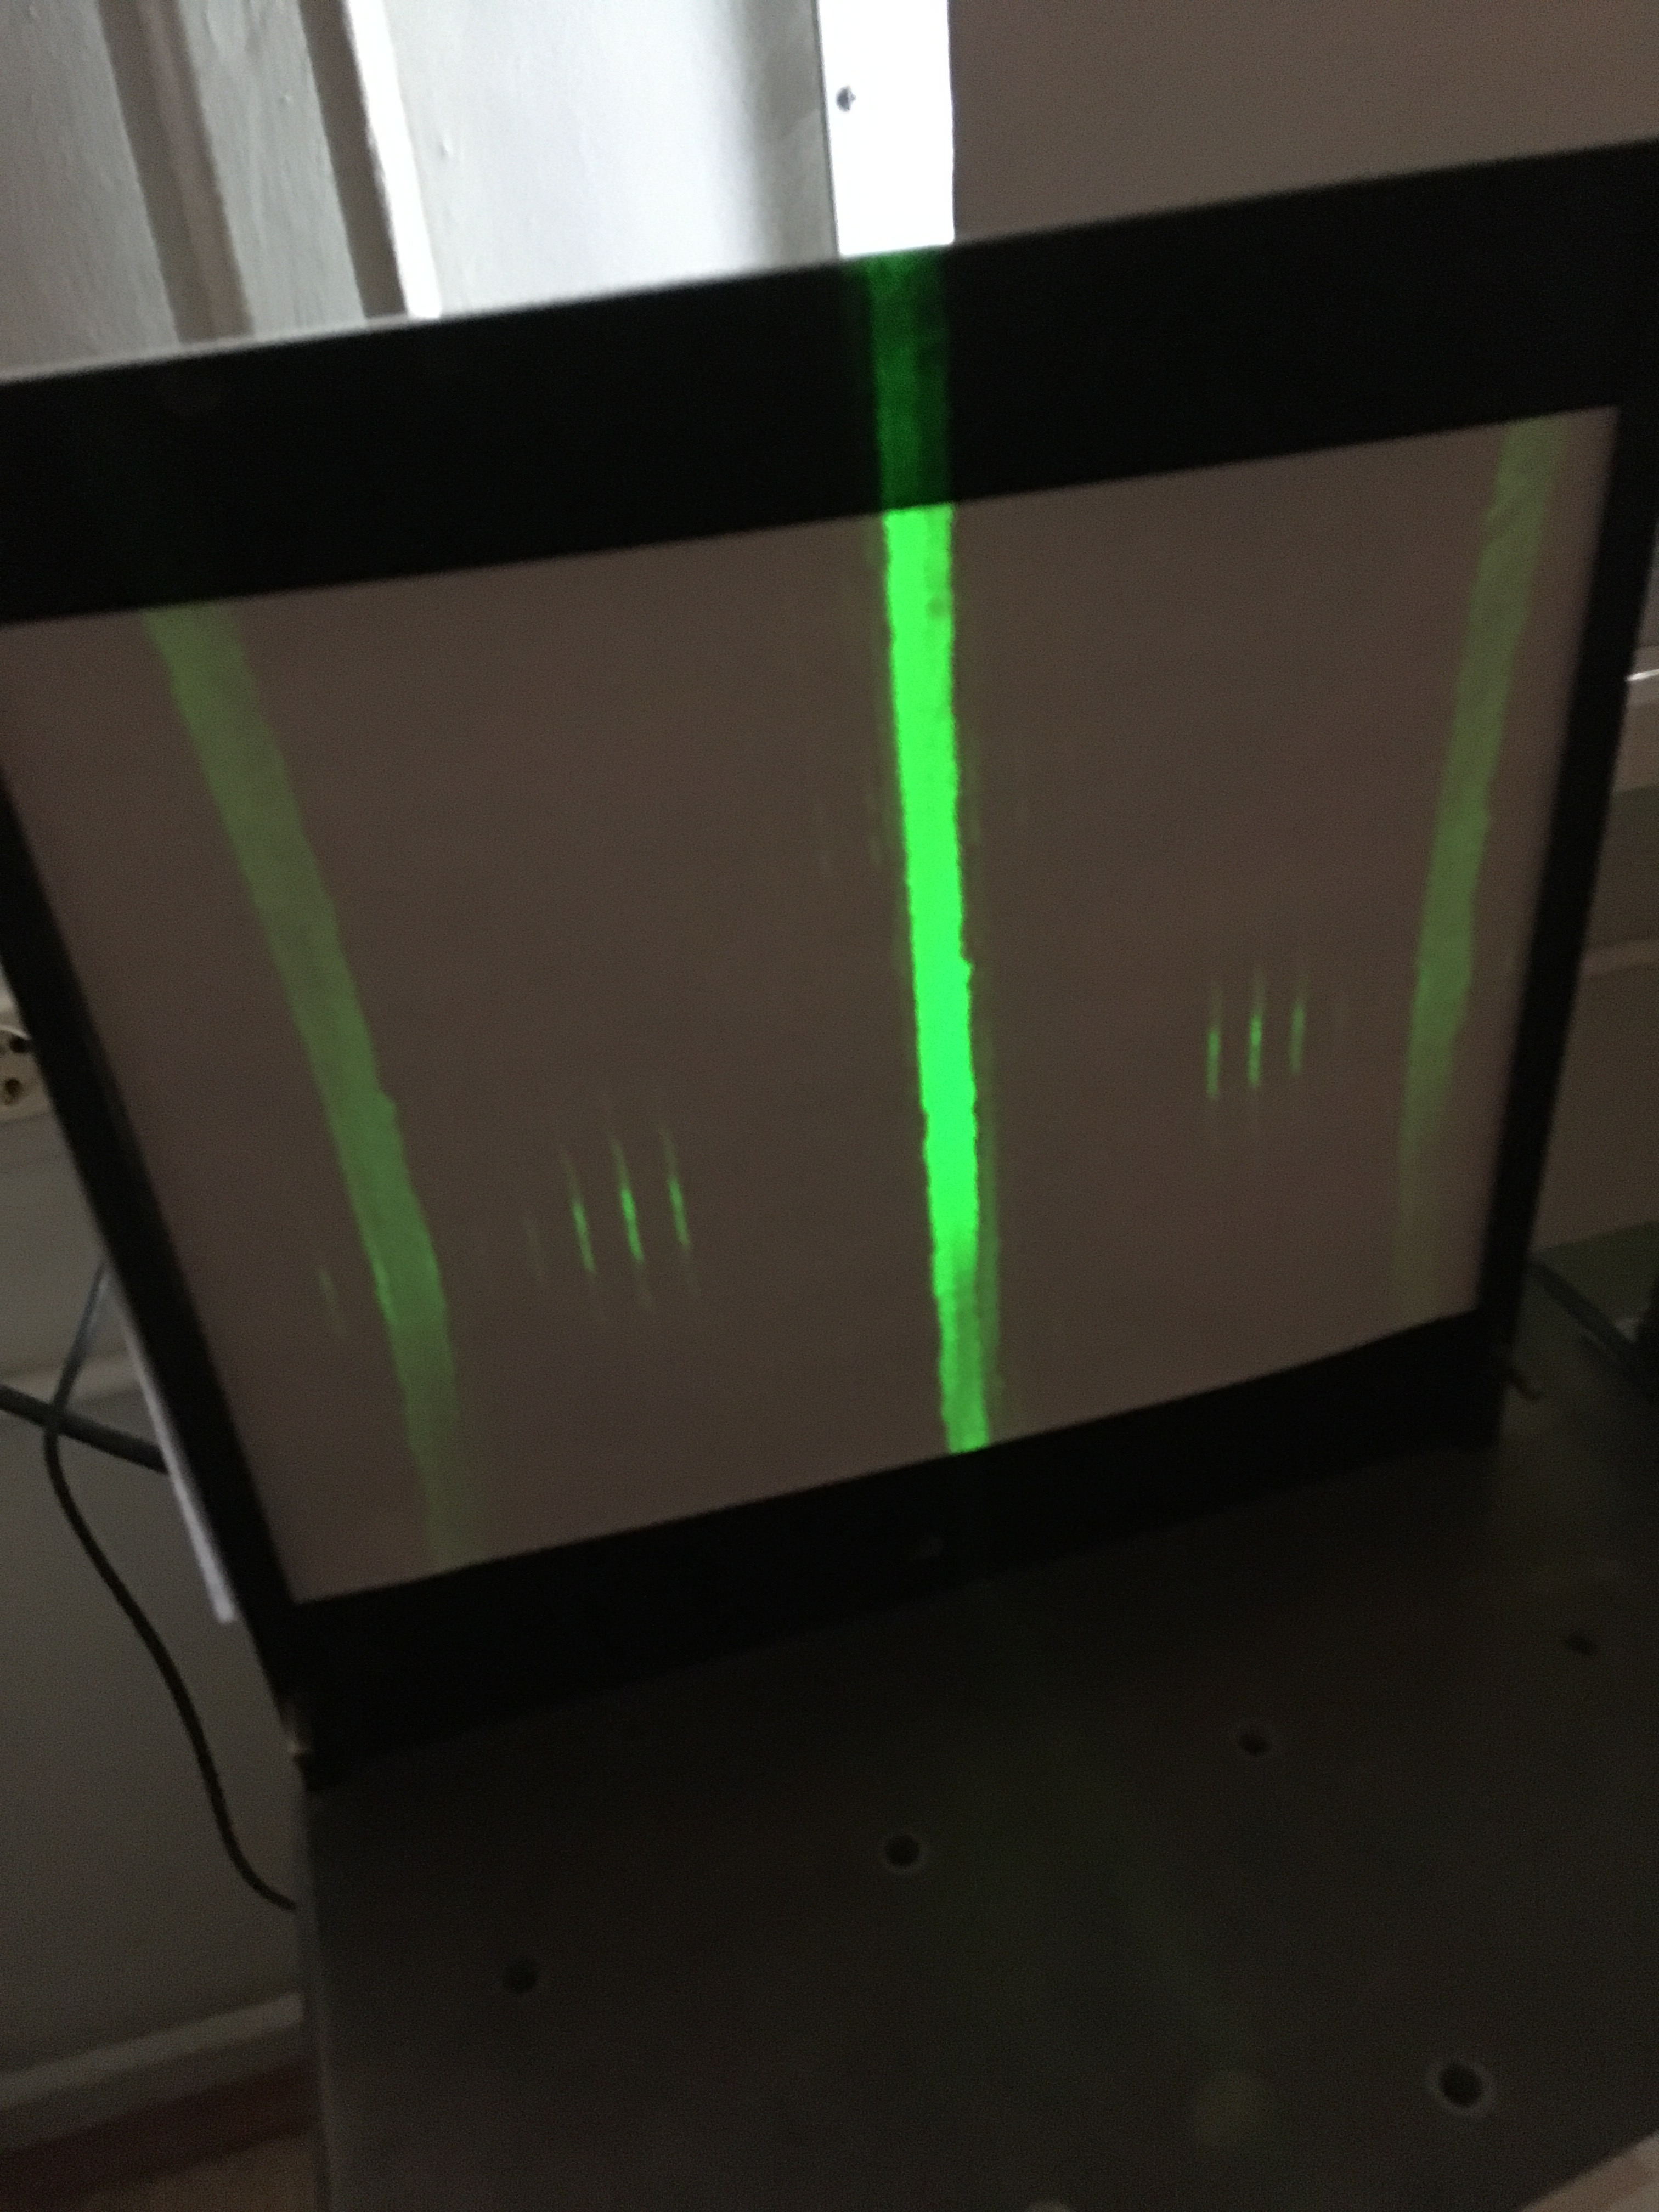
\includegraphics[width=0.8\linewidth]{IMG_3270}
	\end{minipage}
	\caption{Мультипликация изображения щели при разных периодах решётки}
	\label{fig:мультипликация}
\end{figure}
\newpage
\subsection{Сравнение результатов и оценка погрешностей}

Добавим все полученные периоды решётки в сводную таблицу \ref{tab:Сводная}. Можно видеть, что данные, полученные по изображению, не совпадают с остальными и имеют б\'{о}льшую погрешность. Это связано с общими недостатками метода, например, с погрешностью определения фокусного расстояния (изображение может быть достаточно чётким на довольно большом диапазоне расстояний) и др.

\begin{table}[h]
	\centering
	\begin{tabular}{|l|l|l|l|}
		\hline
		\multicolumn{1}{|c|}{\multirow{2}{*}{$n$}} & \multicolumn{3}{c|}{d, мм}                              \\ \cline{2-4} 
		\multicolumn{1}{|c|}{}                     & По спектру       & По изображению  & По мин. разрешению \\ \hline
		2                                          & $0.0198\pm 1E-4$ & ---             & ---                \\ \hline
		3                                          & $0.0302\pm 3E-4$ & $0.04\pm 0.01$  & $0.0349\pm 1E-4$   \\ \hline
		4                                          & $0.060\pm 0.001$ & $0.07\pm 0.01$  & $0.0600\pm 3E-4$   \\ \hline
		5                                          & $0.120\pm 0.005$ & $0.14\pm 0.015$ & $0.117\pm 0.001$   \\ \hline
		6                                          & $0.16\pm 0.01$   & $0.18\pm 0.02$  & $0.168\pm 0.003$   \\ \hline
	\end{tabular}
	\caption{Сводная таблица результатов измерений периода $d$.}
	\label{tab:Сводная}
\end{table}

Как и обычно, погрешности вычисляются по общей формуле. Погрешность фокусного расстояния линз взята равной единице младшего разряда. 

Стоит заметить, что в 3-м опыте указанная погрешность несколько меньше фактической, т. к. критерий Рэлея обычно не даёт достаточно точных результатов, а микрометрический винт имеет достаточно небольшую инструментальную погрешность. Для увеличения точности опыт был проведён дважды. В расчёт брались только усреднённые значения.

\subsection{Проверка теории Аббе}

Для проверки построим график $ d = f(1/D) $ на рис. \ref{fig:screenshot4}
\begin{figure}[tb]
	\centering
	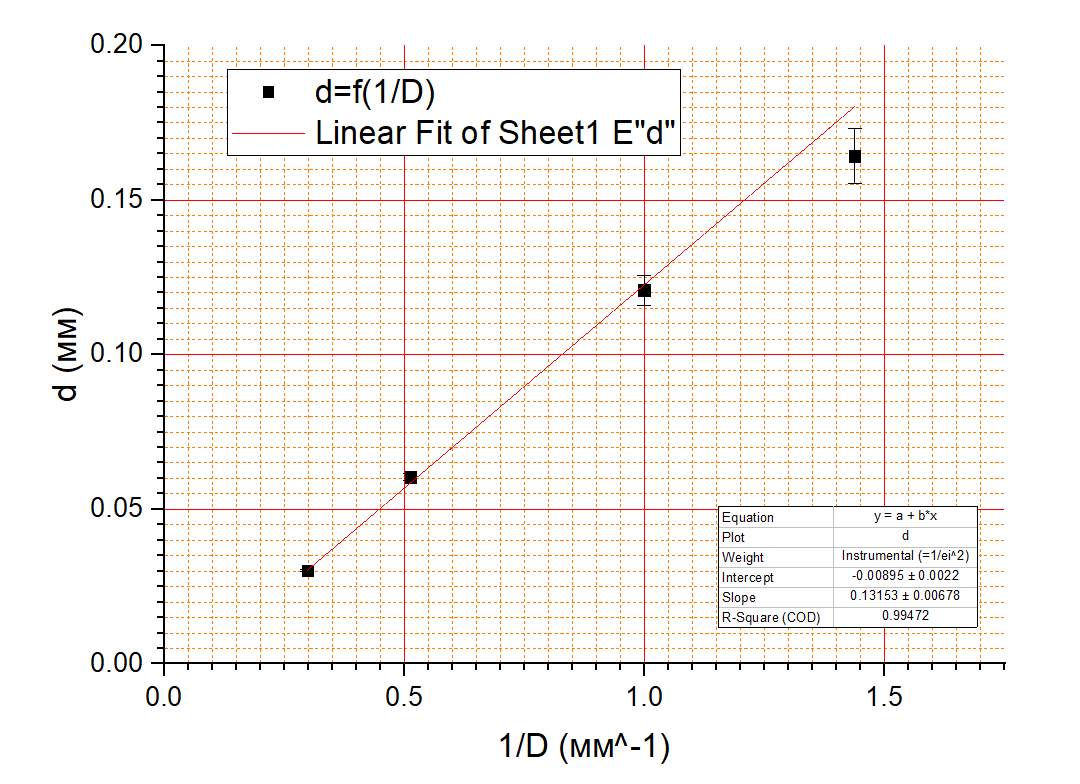
\includegraphics[width=0.8\linewidth]{Screenshot_4}
	\caption{График зависимости $d(1/D)$}
	\label{fig:screenshot4}
\end{figure}
и найдём коэффициент $$ k_{эксп} = 0.13\pm 0.01. $$ Посчитаем точный коэффициент: $$ k_{точн} = 2 f \lambda = 0.12, $$ что совпадает в рамках погрешности. В пределах этих опытов теория Аббе выполняется.

\section{Вывод}

Определили несколькими способами периоды решёток; исследовали зависимость дифракционного предела разрешения объектива микроскопа от его диаметра; на качественном уровне изучили пространственную фильтрацию и мультипликацию изображения решётки.

\begin{thebibliography}{9}
	\bibitem{Siv} Сивухин Д. В. \emph{Общий курс физики. Том 4 Оптика}, 2004
	\bibitem{kir} Кириченко Н. А. \emph{Принципы оптики}, 2014
	\bibitem{max} \emph{Лабораторный практикум по общей физике. В 3 томах. Том 2. Оптика: учебное пособие} под ред. А. В. Максимычева
\end{thebibliography}
\end{document}